% Template for Cogsci submission with R Markdown

% Stuff changed from original Markdown PLOS Template
\documentclass[10pt, letterpaper]{article}

\usepackage{cogsci}
\usepackage{pslatex}
\usepackage{float}
\usepackage{caption}

% amsmath package, useful for mathematical formulas
\usepackage{amsmath}

% amssymb package, useful for mathematical symbols
\usepackage{amssymb}

% hyperref package, useful for hyperlinks
\usepackage{hyperref}

% graphicx package, useful for including eps and pdf graphics
% include graphics with the command \includegraphics
\usepackage{graphicx}

% Sweave(-like)
\usepackage{fancyvrb}
\DefineVerbatimEnvironment{Sinput}{Verbatim}{fontshape=sl}
\DefineVerbatimEnvironment{Soutput}{Verbatim}{}
\DefineVerbatimEnvironment{Scode}{Verbatim}{fontshape=sl}
\newenvironment{Schunk}{}{}
\DefineVerbatimEnvironment{Code}{Verbatim}{}
\DefineVerbatimEnvironment{CodeInput}{Verbatim}{fontshape=sl}
\DefineVerbatimEnvironment{CodeOutput}{Verbatim}{}
\newenvironment{CodeChunk}{}{}

% cite package, to clean up citations in the main text. Do not remove.
\usepackage{apacite}

% KM added 1/4/18 to allow control of blind submission


\usepackage{color}

% Use doublespacing - comment out for single spacing
%\usepackage{setspace}
%\doublespacing


% % Text layout
% \topmargin 0.0cm
% \oddsidemargin 0.5cm
% \evensidemargin 0.5cm
% \textwidth 16cm
% \textheight 21cm

\title{Words aren't created equal: Investigating bias on the CDI}


\author{{\large \bf Morton Ann Gernsbacher (MAG@Macc.Wisc.Edu)} \\ Department of Psychology, 1202 W. Johnson Street \\ Madison, WI 53706 USA \AND {\large \bf Sharon J.~Derry (SDJ@Macc.Wisc.Edu)} \\ Department of Educational Psychology, 1025 W. Johnson Street \\ Madison, WI 53706 USA}

\newlength{\cslhangindent}
\setlength{\cslhangindent}{1.5em}
\newenvironment{CSLReferences}%
  {}%
  {\par}

\begin{document}

\maketitle

\begin{abstract}
Children's early language skill has been linked to later educational
outcomes, making it important to accurately measure early language.
Parent-reported instruments such as the Communicative Development
Inventories (CDIs) have been shown to provide valid, consistent measures
of children's aggregate early language skill. However, CDIs are
predominantly comprised of hundreds of vocabulary items, some of which
may not be heard (and thus learned) equally often by children of varying
backgrounds. Here, we use a database of American English CDIs to
identify words that show strong bias for particular groups of children,
along the axes of sex (male vs.~female), race/ethnicity (white
vs.~non-white), and socioeconomic status (high vs.~low). For each axis,
we identify dozens of strongly biased items, and show that eliminating
these items reduces the expected ability difference between groups. For
sex, we consider how to propose replacement words that may show less
bias, on the basis of their relatively equal frequency in adult speech
directed to male and female children.

\textbf{Keywords:}
language acquisition; word learning; measuring instrument bias;
development;
\end{abstract}

\hypertarget{introduction}{%
\section{Introduction}\label{introduction}}

Researchers, clinicians, and parents have long been fascinated with the
surprising speed and variability in the growth of young children's
vocabulary. Children's early vocabulary growth is assumed to reflect not
only their exposure to child-directed speech, but also the varying
difficulty of different types of words, and individual differences in
the aptitude of the child -- including potential language deficits.
Research has uncovered both within-child consistency in development, as
well as significant influence from external factors. For example,
Bornstein, Hahn, \& Putnick (2016) found stability in core language
skills across 10 years of children's development, despite changes in
maternal income and education over the study period. Yet socioeconomic
status (SES) has also been found to be predictive of children's early
language skill, and of later educational outcomes (for a review, see
Schwab \& Lew-Williams, 2016). Biological factors are also predictive of
language skill: first-born children tend to outpace their siblings, and
female children tend to have better language skills than their
age-matched male counterparts (Larry Fenson et al., 1994) -- an
sex-based verbal advantage that continues through high school (see
Petersen, 2018 for a review). However, it is also difficult to measure
language skill: in any short recording children are unlikely to use all
of the words and constructions that they know, and any comprehensive
battery of language measures will likely exhaust children's attention
span.

The MacArthur-Bates Communicative Development Inventories {[}CDIs; L.
Fenson et al. (2007){]} are a set of parent-reported measures of
children's productive and receptive language skills, which produce a
low-cost and reliable way to estimate children's early language skills
(Larry Fenson et al., 1994). CDIs have shown good predictive validity
{[}e.g., Larry Fenson et al. (1994); Bornstein et al.~2012, Duff et
al.~2015{]}. Our focus will be on the vocabulary checklist portion of
the CDI Words \& Sentences (CDI:WS) form, comprised of 680 early-learned
words across 22 categories (e.g., animals, vehicles, action words,
pronouns) selected to assess the productive vocabulary of children 16 to
30 months of age. For each item on the CDI:WS, caregivers are asked to
respond whether the target child has been heard to say (i.e.~produce)
the given item.\footnote{The CDI: Words and Gestures form includes a
  subset of the CDI:WS items and targets children 12 to 18 months of
  age, measuring both comprehension and production.} Children's total
vocabulary score on the CDI:WS is tightly correlated with other facets
of early language (e.g., grammatical competence and gesture), suggesting
that the language system is ``tightly woven'' (Frank, Braginsky,
Yurovsky, \& Marchman, 2021). Due to these desirable properties, CDIs
have been adapted to dozens of languages, and a central repository of
CDI data contributed from all over the world has been created
{[}Wordbank; Frank, Braginsky, Yurovsky, \& Marchman (2017); Frank,
Braginsky, Yurovsky, \& Marchman (2021){]}.

Inspired by the utility and widespread use of the CDI, researchers have
recently been using psychometric models on CDI data to construct short,
adaptive tests to reliably assess language ability using only a small
subset of the CDI items Kachergis, Marchman, Dale, Mankewitz, \& Frank
(2021). These psychometric models typically come from the Item-Response
Theory (IRT) framework (Baker, 2001), which assumes that not only
test-takers (here, children) have normally-distributed ability, but that
items (words on the CDI) have normally-distributed difficulty. The very
efficacy of these IRT-based models depends on words varying in
difficulty, and hence being more/less informative of the ability level
of different individuals. For example, asking whether a 22-month-old
produces the word ``ball'' is far less informative of that child's
language ability than asking whether they produce ``table,'' as 96\% of
22-month-olds can produce the former, while only 47\% produce the
latter.

While it is quite reasonable to expect that some CDI words are easier
than others, and even to use these varying difficulties to predict
variation in children's language ability, the use of psychometric models
highlights the possibility that some CDI items may function differently
(i.e., be more/less difficult) for different groups of children. The
idea that some items on a test may show bias, favoring one group over
another, is known as Differential Item Function (DIF; Holland \& Wainer
(1993){]}. A variety of statistical methods for detecting DIF have been
proposed, and investigations have in several instances identified DIF
for many items on tests favoring particular one group over another
(e.g., rural vs.~urban). Our goal here is to test the items on the
American CDI:WS for DIF along three main axes: sex (male vs.~female),
socioeconomic status (low- vs.~high-SES), and ethnicity (white
vs.~non-white).

We take the approach put forward by Stenhaug, Frank, \& Domingue (2021):
GLIMMER plots based on the 1-parameter logistic are sufficient to
identify bias, without potentially obscuring DIF in a more complex
model's additional parameters.

DIF is, however, a challenging metric for identifying bias for a couple
reasons. Firstly, DIF is extremely hard to accurately root out. The
process of finding DIF involves using the test you used to do IRT
analysis in order to look for bias within the very same test. Secondly,
the presence of DIF does not necessarily indicate the presence of bias;
it can indicate that one demographic has a higher average ability level
than the other. These two issues are the basis upon which we get the
Fundamental DIF Identification problem.

This problem can be be understood through a concrete example that is
well-known from research on early language learning: consider the fact
that females show a larger vocabulary than males across early
development {[}see Frank, Braginsky, Yurovsky, \& Marchman (2021) Ch.
6?; OTHER REFS{]}. The question is whether or not females actually have
a higher ability level, or if the tests predominantly have words that
are easier for females (i.e., biased). (It could even be that the test
is biased toward males but the language ability of females is large
enough to overcome that bias.) To address this question, we need to know
the ability levels of girls and boys in order to confirm that if a word
is learned earlier by girls it is simply because of an ability
difference rather than a bias inherent to the word. The problem arises
from the fact that we measure ability level using the very same test
that we are trying to check for biased words. If the boys and girls were
of the same average language ability, this would not be an issue but
given the evidence showing that girls have a higher ability level, we
need to know the difference in ability so that when we find DIF for a
specific word can be sure it is outside of the expecting DIF that
results naturally from their difference in ability.

The outline of this paper is as follows. First, we will introduce the
Wordbank data and the IRT model we use to analyze the data.

\hypertarget{methods}{%
\section{Methods}\label{methods}}

\hypertarget{vocabulary-data}{%
\subsection{Vocabulary Data}\label{vocabulary-data}}

\hypertarget{participants}{%
\subsubsection{Participants}\label{participants}}

We analyze parent-reported Wordbank data from 5520 American English CDI:
Words \& Sentences administrations for children 16 to 30 months of age
(Frank, Braginsky, Yurovsky, \& Marchman, 2017, 2021). Full demographic
data are not reported in some datasets contributed to Wordbank: sex is
available for 4094 children, 4094.

We focused on comparing data between demographic groups on the axes of
Sex, Ethnicity and Mother's Education, a proxy for socioeconomic status
(henceforth, SES). Our data included 1989 female and 2105 male
participants. In terms of Ethnicity data was recorded from 2202 white,
67 Asian, 222 Black, 131 Hispanic, and 93 ``Other'' participants as well
as 2805 unreported. Given our distribution of ethnicities, for our
analysis we split participants into White (2202) and Non-White (513).
Finally, we split participants into high and low SES, of which we had
4973 high SES participants, corresponding to mothers' education of some
college or higher and 547 Low SES participants.

\hypertarget{rasch-model}{%
\subsection{Rasch Model}\label{rasch-model}}

The Rasch model, also known as the 1-parameter logistic (1PL) model, is
the simplest Item Response Theory model, and is thus the easiest to use
to investigate potential differences in item function across different
groups of participants. The goal of the Rasch model is to jointly
estimate for each child \(j\) a latent ability \(\theta_j\), and for
each item \(i\) a difficulty parameter \(b_i\). In the model, the
probability of child \(j\) knowing (i.e., producing or understanding) a
given item \(i\) is

\[P_{i}(x_i = 1 | b_{i},\theta_j ) = \frac{1}{1 + e^{-D(\theta_j - b_i )}}\]

where \(D\) is a constant scaling parameter (\(D=1.702\)) which makes
the logistic closely match the ogive function in traditional factor
analysis (Chalmers, 2012; Reckase, 2009). Child ability (\(\theta\)) and
item difficulty (\(b\)) distributions are standardized (i.e., mean of
0), and expected to be normally-distributed. Children with high latent
ability (\(\theta\)) will be more likely to produce any given item than
children with lower latent ability, and more difficult items will be
produced by fewer children (at any given \(\theta\)) than easier items.

In the multigroup Rasch model, an item's difficulty is allowed to vary
depending on which group an individual child belongs to. For example, in
the sex-based multigroup model, item \(i\)'s difficulty is
\(b_{i}^{female}\) for females, and \(b_{i}^{male}\) for males. We
fitted a multigroup Rasch model for each demographic dimension (sex,
socioeconomic status, and ethnicity).

\hypertarget{results}{%
\section{Results}\label{results}}

\begin{CodeChunk}
\begin{figure}[H]

{\centering 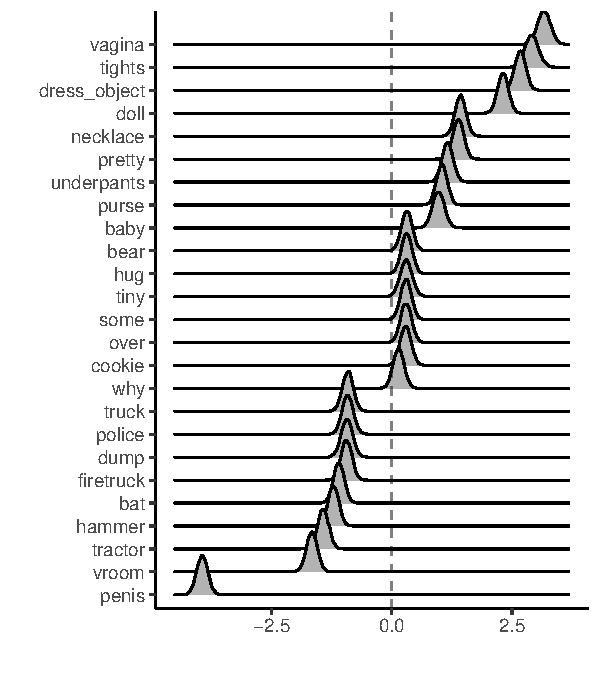
\includegraphics[width=\linewidth]{figs/smGLIMMER_sex_prodWS} 

}

\caption[GLIMMER plot of a sample of CDI:WS words from the sex bias model]{GLIMMER plot of a sample of CDI:WS words from the sex bias model. Words at the top are easier to learn for females, while those at the bottom are easier for males.}\label{fig:sex-glimmer}
\end{figure}
\end{CodeChunk}

\begin{CodeChunk}
\begin{figure}[H]

{\centering 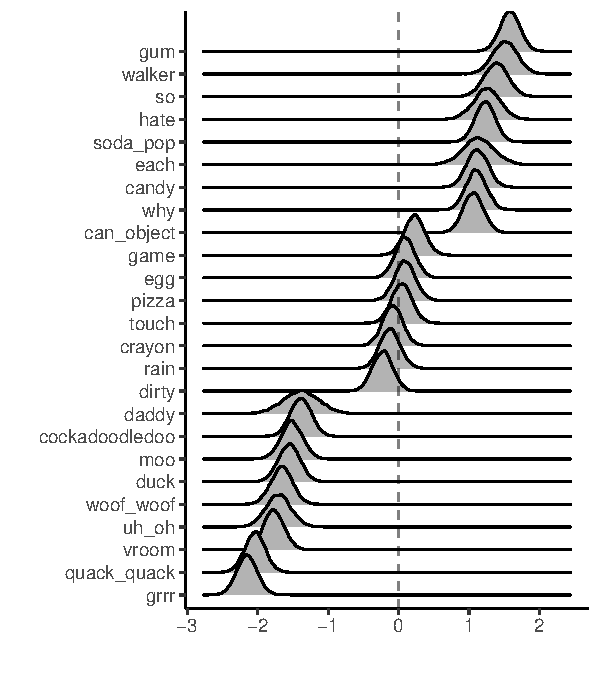
\includegraphics[width=\linewidth]{figs/smGLIMMER_ses_prodWS} 

}

\caption[GLIMMER plot of a sample of CDI:WS words from the SES bias model]{GLIMMER plot of a sample of CDI:WS words from the SES bias model. Words at the top are easier to learn for children from low-SES families, while those at the bottom are easier for those from high-SES families.}\label{fig:ses-glimmer}
\end{figure}
\end{CodeChunk}

\begin{CodeChunk}
\begin{figure}[H]

{\centering 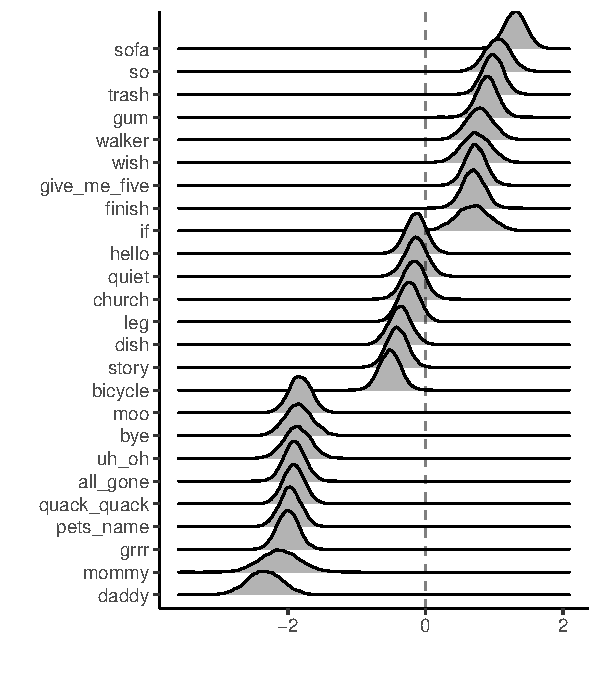
\includegraphics[width=\linewidth]{figs/smGLIMMER_eth_prodWS} 

}

\caption[GLIMMER plot of a sample of CDI:WS words from the ethnicity bias model]{GLIMMER plot of a sample of CDI:WS words from the ethnicity bias model. Words at the top are easier to learn for children from low-SES families, while those at the bottom are easier for those from high-SES families.}\label{fig:eth-glimmer}
\end{figure}
\end{CodeChunk}

\hypertarget{discussion}{%
\section{Discussion}\label{discussion}}

\hypertarget{acknowledgements}{%
\section{Acknowledgements}\label{acknowledgements}}

Place acknowledgments (including funding information) in a section at
the end of the paper.

\hypertarget{references}{%
\section{References}\label{references}}

\setlength{\parindent}{-0.1in} 
\setlength{\leftskip}{0.125in}

\noindent

\hypertarget{refs}{}
\begin{CSLReferences}{1}{0}
\leavevmode\hypertarget{ref-Baker2001}{}%
Baker, F. B. (2001). \emph{The basics of item response theory}. ERIC.

\leavevmode\hypertarget{ref-bornstein2016stability}{}%
Bornstein, M. H., Hahn, C.-S., \& Putnick, D. L. (2016). Stability of
core language skill across the first decade of life in children at
biological and social risk. \emph{Journal of Child Psychology and
Psychiatry}, \emph{57}(12), 1434--1443.

\leavevmode\hypertarget{ref-R-mirt}{}%
Chalmers, R. P. (2012). {mirt}: A multidimensional item response theory
package for the {R} environment. \emph{Journal of Statistical Software},
\emph{48}(6), 1--29.
http://doi.org/\href{https://doi.org/10.18637/jss.v048.i06}{10.18637/jss.v048.i06}

\leavevmode\hypertarget{ref-fenson1994}{}%
Fenson, Larry, Dale, P. S., Reznick, J. S., Bates, E., Thal, D. J.,
Pethick, S. J., \ldots{} Stiles, J. (1994). Variability in early
communicative development. \emph{Monographs of the Society for Research
in Child Development}, i--185.

\leavevmode\hypertarget{ref-Fenson2007}{}%
Fenson, L., Marchman, V. A., Thal, D. J., Dale, P. S., Reznick, J. S.,
\& Bates, E. (2007). \emph{{M}ac{A}rthur-{B}ates {C}ommunicative
{D}evelopment {I}nventories: User's guide and technical manual (2nd
ed.)}. Baltimore, MD: Brookes.

\leavevmode\hypertarget{ref-frank2017}{}%
Frank, M. C., Braginsky, M., Yurovsky, D., \& Marchman, V. A. (2017).
Wordbank: An open repository for developmental vocabulary data.
\emph{Journal of Child Language}, \emph{44}(3), 677.

\leavevmode\hypertarget{ref-frank2021}{}%
Frank, M. C., Braginsky, M., Yurovsky, D., \& Marchman, V. A. (2021).
\emph{Variability and consistency in early language learning: The
wordbank project}. MIT Press.

\leavevmode\hypertarget{ref-holland1993differential}{}%
Holland, P. W., \& Wainer, H. (1993). \emph{Differential item
functioning}. Routledge.

\leavevmode\hypertarget{ref-kachergis2021cat}{}%
Kachergis, G., Marchman, V. A., Dale, P., Mankewitz, J., \& Frank, M. C.
(2021). Online computerized adaptive tests (CAT) of children's
vocabulary development in english and mexican spanish.

\leavevmode\hypertarget{ref-mayor2019}{}%
Mayor, J., \& Mani, N. (2019). A short version of the
{M}ac{A}rthur-{B}ates {C}ommunicative {D}evelopment {I}nventories with
high validity. \emph{Behavior Research Methods}, \emph{51}(5),
2248--2255.

\leavevmode\hypertarget{ref-petersen2018gender}{}%
Petersen, J. (2018). Gender difference in verbal performance: A
meta-analysis of united states state performance assessments.
\emph{Educational Psychology Review}. Springer.

\leavevmode\hypertarget{ref-reckase2009}{}%
Reckase, M. D. (2009). Multidimensional item response theory models. In
\emph{Multidimensional item response theory} (pp. 79--112). Springer.

\leavevmode\hypertarget{ref-schwab2016}{}%
Schwab, J. F., \& Lew-Williams, C. (2016). Language learning,
socioeconomic status, and child-directed speech. \emph{WIREs Cognitive
Science}, \emph{7}, 264--275.
http://doi.org/\href{https://doi.org/10.1002/wcs.1393}{10.1002/wcs.1393}

\leavevmode\hypertarget{ref-stenhaug2021treading}{}%
Stenhaug, B., Frank, M. C., \& Domingue, B. (2021). Treading carefully:
Agnostic identification as the first step of detecting differential item
functioning.

\end{CSLReferences}

\bibliographystyle{apacite}


\end{document}
